\section{Paralelismus – využití, paralelní technologie.}
\subsection{Souběžnost vs paralelismus}
Souběžné(Concurrent) programy jsou programy vykonávající úlohy nezávisle na sobě a mohou se odehrávat na jednom jádře.
Paralelní je program právě tehdy když jeden program vykonává více úloh zároveň. Všechny paralelní programy jsou 
souběžné, ale ne všechny souběžné programy jsou paralelní.

\subsection{Využití}
Ne pro všechno je vhodný. Už není možné pokračovat s trendem Moorova zákona (každých několik let se zdvojnásobí počet tranzistorů
v integrovaných čipech). Je nutné využít více jader pro zvýšení výkonnosti. Zvyšování frekvence vyžaduje vyšší napájení a jak 
takový čip chladit?

Příklady využití: 
\begin{itemize}
    \item Simulace
    \item Renderování grafiky a grafické zpracování
    \item Big data
    \item AI
\end{itemize}

\subsection{Paralelní technologie}
\begin{itemize}
    \item CPU (vícejádrový / vícevláknový (hyperthreading))
    \item GPU
    \item Distribuované systémy - clustery, grid computing, cloud computing
\end{itemize}

\section{CPU – návrh paralelního programu, vlákna a procesy, synchronizace dat (Lock, RLock, Semaphore).}
\subsection{Návrh paralelního programu}
\begin{itemize}
    \item Nalezení částí, které mohou být paralelizovány
    \item Rozdělení úloh do vláken/procesů
    \item Ošetření přístupu ke sdíleným datům
    \item Ošetření deadlocků a race conditions
\end{itemize}

\subsection{Vlákna a~procesy}
Procesy mají vlastní paměťový prostor (kontext). Vlákna tento kontext mezi sebou sdílí, jeden proces může mít více vláken.

\subsubsection{Procesy}
Každý proces má svůj vlastní paměťový prostor (halda a datové segmenty). Procesy mezi sebou nesdílí paměť. Mohou mezi sebou komunikovat pomocí meziprocesové komunikace(IPC) pomocí front, socketů, rour.  Nové procesy se vytváří pomocí \texttt{fork()}, \texttt{popen()} nebo \texttt{system()}. Child procesy běží nezávisle na rodičovském procesu.

\subsubsection{Vlákna}
Jsou součástí procesu a sdílí celý paměťový prostor procesu. Je to softwarová abstrakce, která umožňuje provádění více souběžných operací na stejných datech. Vlákna mohou být plně souběžná. 
Jejich použití je vhodné pro obsluhu I/O. Mimo sdíleného prostoru mají i svůj vlastní paměťový prostor v podobě zásobníku a registrů. Zásobník vs halda - zásobník pevná velikost, alokace/dealokace změnou pointeru, halda proměnná velikost, doalokování/odalokování paměti podle potřeby. Zásobník ukládá dočasná lokální data do RAM, registry obsahují návratové adresy, stav programu, mezivýsledky apod. Je nutné vlákna synchronizovat, aby nedošlo k inkonzistencím v paměti (moment, kdy 2 vlákna operují nad stejnou pamětí), tzv. mutual exclusion (mutex).
\begin{figure}[ht]
    \centering
    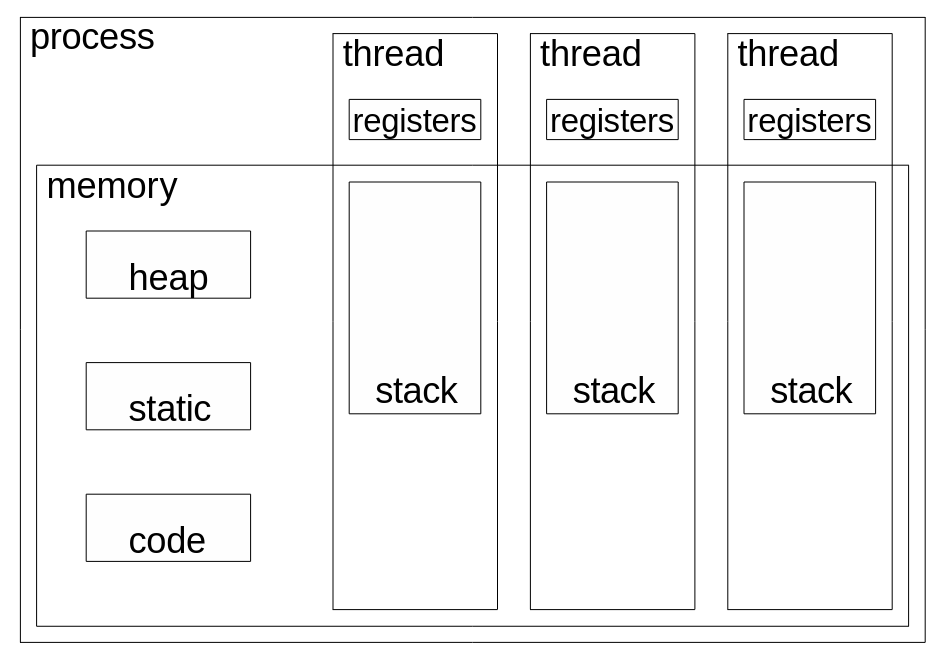
\includegraphics[width=0.5\linewidth]{pict/multithread.png}
    \caption{Multi-threaded proces}
\end{figure}

Python je debílek, protože má GIL (Global Interpreter Lock) a z jednoho procesu může běžet jenom jedno vlákno. Má 2 knihovny, low-level \texttt{thread} (jednoduché mutex locks, vytváření threadů, zabíjení threadů, signály může chytat jenom hlavní vlákno) a high-level \texttt{threading} (víc locků, lepší fíčury). Stavy python vláken: inital state (před startem), runnable(po startu, ale čeká na místo v procesoru), running(když scheduler vybere vlákno k tomu aby dělalo bžum bžum), blocked (čeká na zdroje využívané jiným vláknem), dead(když run() metoda doběhne. Jádro se zničí a nemůže být provedeno znovu.)

\subsection{Lock}
\begin{itemize}
    \item Jedná se o~zámek kritické sekce. 
    \item 2 stavy: zamčeno, odemčeno
    \item Pokud se zámek snaží získat vlákno:
    \begin{itemize}
        \item Pokud je zámek odemčený, zamkne ho vlákno pro sebe
        \item Pokud je zámek zamčený, vlákno je blokováno, dokud se zámek neuvolní
    \end{itemize}
\end{itemize}

\subsection{RLock}
\begin{itemize}
    \item Podobný jako Lock, ale R znamená \uv{reentrant}, další volání stejného vlákna na získání zámku toto vlákno nezablokuje
    \item Je potřeba zámek uvolnit stejně-krát jako byl získán
    \item Vhodné pro rekurzivní funkce
\end{itemize}

\subsection{Semaphore}
\begin{itemize}
    \item Umožňuje určitý počet přístupů
    \item Každé vlákno, které semafor získá, dekrementuje počítadlo
    \item Pokud vlákno chce získat přístup k~semaforu, s~počítadlem na nule, je blokované, dokud některé předchozí vlákno semafor neuvolní
    \item Vhodné pro limitování  počtu vláken, které mají přístup k~nějakému zdroji (třeba socket)
\end{itemize}


\section{GPU – vztahy mezi vlákny, bloky a mřížkou (grid), charakteristika Streaming Multiprocesoru.}
\subsection{Vlákno}
\begin{itemize}
    \item Vlákno provádí jedny instrukce (kernel) nad jednou částí dat
    \item Seskupení do Warpů: 32 jader má stejnou instrukci, ale různá data
    \item Warpy jsou lock-step (dělají stejné kroky ve stejný čas)
    \item SIMT (single instruction set, multiple threads) všechny vlákna ve warpu vykonávají stejnou instrukci, ale s jinými daty
    \item Žadný context switching, každé vlákno má své registry, jejich velikost limituje počet vláken
    \item Má \texttt{threadIdx}, které může být 1D až 3D
\end{itemize}

\subsection{Bloky}
\begin{itemize}
    \item Skupina vláken, sdílí instrukce~a data
    \item Vykonáván na jediném SM
    \item Má \texttt{blockIdx}, které může být 1D až 3D
    \item Mohou se umisťovat do fronty bloků, ty se pak rozdělují na SM
\end{itemize}

\subsection{Mřížka}
\begin{itemize}
    \item Skupina bloků
    \item Sdílet data mezi bloky lze jedině přes globální paměť (velká a~pomalá)
\end{itemize}

\subsection{Streaming Multiprocessor}
Základní stavební blok GPU, základní blok pro provádění paralelních výpočtů. 
Popis Nvidia GV100 (jedna z~možných architektur)
\begin{itemize}
    \item Jádra FP32 (64 ks), FP64 (32 ks), INT32 Jádra, L1 shared memory, Register files
    \item Rozdělen na 4 procesní bloky, každý má čtvrtinu jader, registry, warp scheduler, L0 instruction cache\dots
    \item Warp (32 vláken) se posílá na vybraná jádra SM
    \item L1 cache (jedna na SM) rozdělena na instrukční a~datovou
    \item Grafické karty mají desítky až stovky SM
\end{itemize}

\begin{figure}[ht]
    \centering
    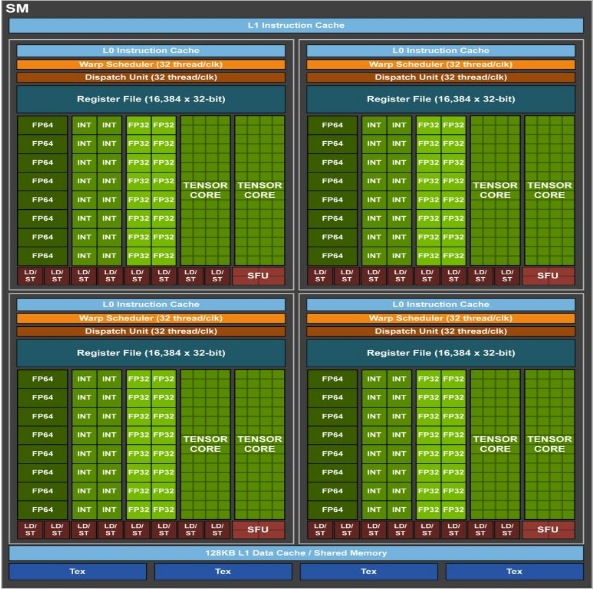
\includegraphics[width=0.7\linewidth]{pict/SM.png}
    \caption{SM}
    \label{fig:SM}
\end{figure}

\section{GPU – paměti – rychlost, velikost, použití (vlákno, blok, mřížka).}
GPU má vlastní DRAM, je menší než DRAM v~PC, ale je do ní rychlejší přístup.

\begin{figure}
    \centering
    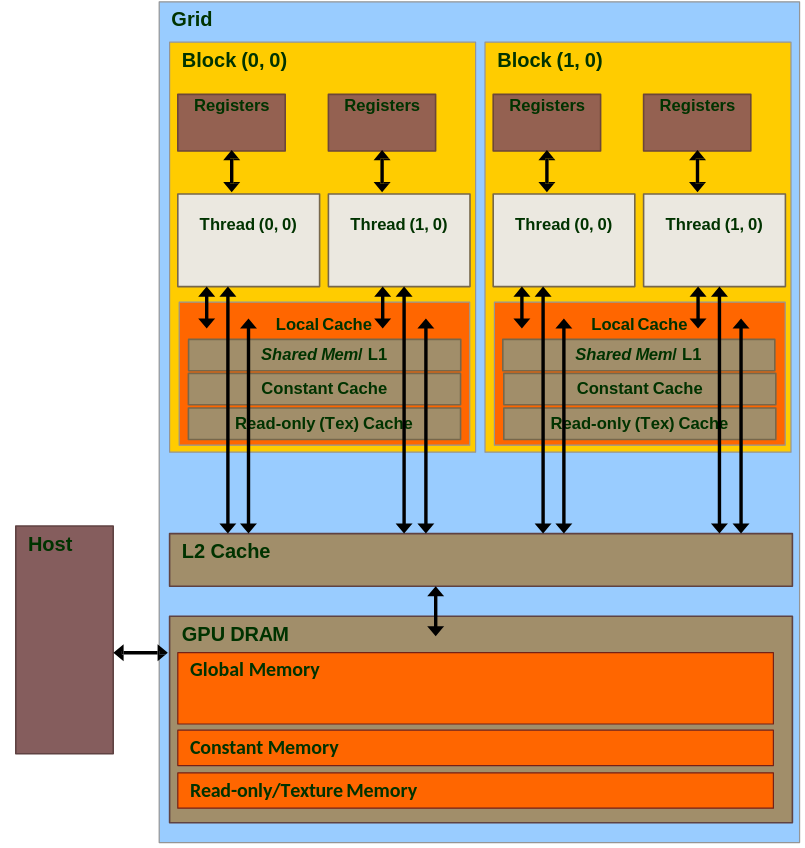
\includegraphics[width=0.6\linewidth]{pict/mem.png}
    \caption{Paměť v GPU}
    \label{fig:enter-label}
\end{figure}
\subsection{Registry}
\begin{itemize}
    \item Nejrychlejší
    \item Nejmenší
    \item Přímo v~SM
    \item Přístup z~vlákna
    \item Rychlý přístup
    \item Stovky KB na SM (jsou jich tisíce, každý má 32 b)
    \item Vlákno může mít proměnlivý počet registrů, maximum dané architekturou
    \item Ukládá data přímo relevantní k~aktuální instrukci
\end{itemize}

\subsection{Lokální (L1) cache}
\begin{itemize}
    \item V~SM
    \item Obsahuje:
    \begin{itemize}
        \item Paměť sdílenou v~bloku (keyword \texttt{\_\_shared\_\_})
        \item Cache konstantní paměti
        \item Cache dat pro čtení
    \end{itemize}
    \item Řádky o~velikosti 128 B (vejde se 32 čísel o délce 32 b)
    \item Přístup z~bloku nebo z~vlákna
    \item Asi 80 cyklů potřeba pro přístup k~paměti
    \item Desítky kB (podle architektury)
    \item Obsahuje taky data pouze pro čtení
\end{itemize}

\subsection{L2 Cache}
\begin{itemize}
    \item Lze sdílet i~mezi bloky (přístup z~celé mřížky)
    \item 6 MB
    \item Stovky cyklů potřebných k~přístupu, až 1000 GB/s bandwidth
    \item \texttt{\_\_global\_\_} keyword
\end{itemize}

\subsection{Lokální paměť}
\begin{itemize}
    \item Paměť která se doalokuje z kernelu
    \item Lokální paměť je dostupná pouze vláknu, které si ji zaalokovalo
    \item Každé vlákno exekuující kernel bude mít svoji vlastní lokální paměť
    \item Stejně jako globální paměť je v DRAM a má podobnou latenci
    \item Automaticky se použije při přetečení registrů
\end{itemize}
\subsection{DRAM}
\begin{itemize}
    \item Přístup z~celé mřížky
    \item Obsahuje:
    \begin{itemize}
        \item Globální paměť
        \item Konstantní paměť
        \item Paměť jen pro čtení
    \end{itemize}
    \item Jednotky až desítky GB
    \item Stovky cyklů potřebných k~přístupu, až 500 GB/s bandwidth
    \item GDDR6/7
\end{itemize}

\begin{table}[]
    \centering
    \begin{tabular}{|c|c|c|c|} \hline
        Paměť & Přístup vlákno & Přístup blok & Přístup mřížka \\ \hline
        Registr & Ano & Ne & Ne \\ \hline
        Sdílená paměť & Ano & Ano & Ne \\ \hline
        L2 Cache  & Ano & Ano & Ano \\ \hline
        Globální paměť & Ano & Ano & Ano  \\ \hline
        Konstantní paměť & Ano & Ano & Ano \\ \hline
        Lokální paměť & Ano & Ne & Ne \\ \hline
    \end{tabular}
    \caption{Přístupy do pamětí}
    \label{tab:my_label}
\end{table}

\subsection{Rozdíl mezi konstantní a~pamětí jen pro čtení}
\begin{itemize}
    \item Konstantní paměť, druh cache pro celé SM. Sdílená na všech jádrech na SM. Zapsaná při kompilaci před spuštěním kernelu. Definuje se pomocí \texttt{\_\_constant\_\_} 
    \item Paměť jen pro čtení může obsahovat velké množství dat, uložená v globální paměti a čitelná z read-only cache. Například pro velké pole, do cache bloku se načte jen relevatní část, kterou bude zpracovávat.
\end{itemize}

\subsection{Použití cache}
\begin{itemize}
    \item Je potřeba navrhnout kernel tak, aby vyžadoval paměť co nejblíže (ideálně na jediném řádku cache)
    \item Při nedodržení (třeba při načítání každého tisícátého prvku vektoru) se výkon zpomalí kvůli cache misses
    \item Úplně ideální je, pokud jeden warp využívá data z~jediného řádku cache
\end{itemize}

\section{GPU – synchronizace, warp, divergence warpu, atomické operace.}
\subsection{Synchronizace}
\subsubsection{Synchronizace warpu a bloku}
\begin{itemize}
    \item Všechna vlákna warpu jsou synchronizovaná, všechna vykonávána současně, není potřeba je synchronizovat explicitně.
    \item V bloku lze vlákna synchronizovat funkcí CUDA \texttt{\_\_syncthreads();}, tato funkce tvoří bariéru blokující, dokud všechna vlákna bloku nedoběhnou do této bariéry.
    \item Může nastat deadlock, pokud \texttt{\_\_syncthreads} není dosažen všemi vlákny kvůli větvení.
    \item Pořadí bloků garantováno není. Tudíž nejde předpokládat synchronizaci mezi bloky.
    \item Další synchronizační funkce v bloku:
    \begin{itemize}
        \item \texttt{int \_\_syncthreads\_count(predicate)} -- kolik predikátů je pravdivých
        \item \texttt{int \_\_syncthreads\_and(predicate)} -- vrátí \texttt{true}, pokud jsou všechny predikáty pravdivé
        \item \texttt{int \_\_syncthreads\_or(predicate)} -- vrátí \texttt{true}, pokud jsou aspoň některé predikáty pravdivé
    \end{itemize}
    \item taky existuje \texttt{\_\_threadfence\_block();} -- blokuje, dokud všechna vlákna v~bloku nevidí provedené zápisy v~globální a~sdílené paměti
\end{itemize}

\subsubsection{Synchronizace hostitele (PC) a zařízení (GPU)}
V kódu hosta volání \texttt{context.synchronize()}, zajistí, že všechny asynchronní úlohy jsou dokončeny. Blokuje na straně hosta.

\texttt{\_\_threadfence();} Blokuje vlákna v~bloku, dokud všechna z~nich nevidí změny ve sdílené paměti, nebo blokuje všechna vlákna, dokud nejsou změny v~globální paměti viditelné všem

\subsection{Warp}
\begin{itemize}
    \item 32 threadů
    \item Synchronizované \textit{lock-step} (stejná instrukce v~celém warpu)
    \item Každý blok má 1 nebo více Warpů
    \item Každý warp je plánovaný nezávisle na ostatních
    \item Scheduler preferuje warpy, které mají input přichystaný ke zpracování
    \item Protože warpy mají stejné instrukce, nastávají problémy při větvení
    \item Musí se vykonat obě větve pro celý warp, vlákna se pouze maskují ve větvi, která pro ně není relevantní
    \item Není potřeba warp voting, pokud je větvení jasné už z~kompilace (podmínka podle pevně dané hodnoty)
\end{itemize}

\subsection{Warp divergence}
\begin{itemize}
    \item = různá vlákna warpu vyžadují různé větve kódu
    \item Redukuje výkonnost paralelizace
    \item Nejhorší případ: zpomalení 32\(\times\) (pokud každé vlákno má jinou větev)
    \item Existují predikáty, fungují podobně jako if/else: \texttt{p = (x<0.0); p: z = x-2.0; !p:z= sqrt(x);}, pořád se jedná o~3~instrukce
    \item V rámci warpu také dochází k~\uv{warp voting}, každé vlákno avizuje, kterou větev bude vykonávat. Pokud všechna vlákna warpu vykonávají stejnou větev, je výpočet rychlejší (druhá větev se nepoužije vůbec)
\end{itemize}

\subsection{Atomické operace}
\begin{itemize}
    \item Při zápisu více vláken do jediné proměnné
    \item Čtení i zápis v jediné nedělitelné instrukci, zajistí integritu dat (nenastane souběh, při kterém by byla dříve přečtená hodnota změněna jiným vláknem před zápisem, což by přemazalo výstup druhého vlákna)
    \item \texttt{atomicAdd}
    \begin{itemize}
        \item první atribut je pointer, druhý hodnota k~přičtení
    \end{itemize}
    \item \texttt{atomicExch}
    \begin{itemize}
        \item Uloží hodnotu na adresu pointeru
    \end{itemize}
    \item \texttt{atomicMin}
    \item \texttt{atomicMax}
    \item \texttt{atomicCAS(int *addr, int compare, int val)} -- compare and swap, pokud je hodnota \texttt{compare} stejná jako ta na \texttt{addr}, nahraje tam místo toho \texttt{val} -- dá se použít k~atomickým zámkům
    \item A další
    \item Rychlé pro data ve sdílené paměti, pomalé pro globální paměť
\end{itemize}

\section{GPU - paralelní vzory, paralelní redukce, funkce shfl\_down\_sync(), asynchronní spouštění funkcí.}

\subsection{Paralelní vzory}
\begin{itemize}
    \item Jsou to stavební kameny pro složitější algoritmy
    \item Např.\,Map: aplikuje funkci na všechny prvky listu, snadno paralelizovatelné
    \item Další příklad: Scan (nový vektor, má o 1 méně hodnot, v~každém poli je součet hodnot původního pole po aktuální index)
    \item Stencil výpočet prvků na základě sousedů
    \item Histogram/Binning kategorizace vstupů - nutny atomické operace
\end{itemize}
\subsubsection{Redukce}
\begin{itemize}
    \item = Aplikování asociativního binárního operátoru na všechny prvky, redukování do jediné hodnoty
    \item +, *, max, min\dots
    \item Paralelní redukce: což takhle použít strom? -- redukce po párech (vznikne N/2 hodnot), opakovat, dokud nemám jedinou hodnotu
    \item Chtěli bychom dosáhnout toho, ať je celý wapr buď aktivní nebo neaktivní, chceme mitigovat warp divergenci
    \item Redukce na bloku vyžaduje synchronizaci
    \begin{verbatim}
__global__ void sum_reduction(float *input, float *block_results){
    extern __shared__ int sdata[];
    unsigned int i = blockIdx.x*blockDim.x + threadIdx.x;
    sdata[threadIdx.x] = input[i];
    __syncthreads();
    for (unsigned int stride = blockDim.x/2; stride > 0; stride/=2){
        unsigned int strided_i = threadIdx.x * 2 * stride;
        if (strided_i < blockDim.x){
            sdata[strided_i] += sdata[strided_i + stride]
        }
        __syncthreads();
    }
    if (threadIdx.x == 0) {
        block_results[blockIdx.x] = sdata[0];
    }
}
    \end{verbatim}
    \item Globální redukce je vhodná lokálními redukcemi, které jsou pak stejným sečteny atomickými operacemi
\end{itemize}

\subsection{shfl\_down\_sync()}
\subsubsection{Warp shuffle}
\begin{itemize}
    \item Pro přesun dat v~rámci jediného warpu
    \item Lze užít místo atomických operací, nevyžaduje sdílenou paměť, vlákna čtou registry jiných vláken
    \item Je nutné, aby bylo vlákno, ze kterého chci číst, aktivní, jinak se vrátí nedefinovaná hodnota
\end{itemize}
\subsubsection{Warp voting}
\begin{itemize}
    \item Aktivní vlákna mohou v~rámci warpu vyměňovat info o~podmínkách
    \item \texttt{int all\_sync(mask, condition)} -- True, pokud platí podmínka ve všech aktivních vláknech warpu
    \item \texttt{int any\_sync(mask, condition)} -- True, pokud platí podmínka v~aspoň jednom aktivním vláknu warpu
    \item \texttt{unsigned int ballot\_sync(mask, condition)} -- Vrací číslo, kde bity jsou dané hodnotami jednotlivých hodnot condition z~vláken
    \item Všechny tyto funkce blokují, ale jen aktivní vlákna
\end{itemize}
\subsubsection{Samotná funkce}
\begin{itemize}
    \item Argumenty:
    \begin{itemize}
        \item \texttt{unsigned mask} -- která vlákna se účastní
        \item \texttt{T var} -- proměnná
        \item \texttt{unsigned int delat} -- O kolik kroků dále se dívat na registry, z~těchto registrů čte hodnotu \texttt{var}. Pokud takový index neexistuje, vezme jen svou hodnotu registru
        \item \texttt{int width=warpSize}
    \end{itemize}
    \item Navrací hodnotu proměnné z~jiného registru
    \item Užití: třeba součet v~rámci warpu
\begin{verbatim}
#define FULL_MASK 0xffffffff
global void sum_warp_kernel_shfl_down(int *a)
{
    int local_sum = a[threadIdx.x + blockIdx.x*blockDim.x];
    for (int offset = WARP_SIZE / 2; offset>0; offset /= 2) {
        local_sum += shfl_down_sync(FULL_MASK, local_sum, offset);
    }
    if (threadIdx.x%32 == 0) {
        printf("Warp max is %d", local_sum)
    }
}
\end{verbatim}
\end{itemize}

\subsection{Asynchronní spouštění funkcí}
\begin{itemize}
    \item Synchronní blokuje
    \item Asynchronní neblokuje (spustím a jdu na další krok, ono to asi běží někde na pozadí, snad)
\end{itemize}

\subsubsection{Typy asynchronních funkcí}
\begin{itemize}
    \item Vzniklé v CPU pipeline
    \begin{itemize}
        \item napsáno synchronně, kompilátor vyhodnotil, že větve kódu na sebe nemají vliv a~vytvoří instrukce, které se překrývají pro maximální využití pipeline
    \end{itemize}
    \item CPU threading
    \begin{itemize}
        \item Podobná vlákna běží paralelně na procesoru, důležitá synchronizace
    \end{itemize}
    \item CUDA warp execution
    \begin{itemize}
        \item funkce ve stejném warpu jsou vzájemně synchronní
        \item warpy na SMP jsou spouštěny asynchronně
        \item synchronizace mezi warpy pomocí \texttt{syncthreads()}
        \item synchronní jsou:
        \begin{itemize}
            \item volání kernelu
            \item cudaMemcpy (device to device nebo host to device malých dat)
        \end{itemize}
        \item asynchronní volání jsou blokována:
        \begin{itemize}
            \item při \texttt{deviceSynchronize()}
            \item když má být spuštěn nový kernel
            \item Když se musí kopírovat data z~nebo na kartu
        \end{itemize}
    \end{itemize}
\end{itemize}

\subsubsection{CUDA streamy}
\begin{itemize}
    \item Jedná se o~asynchronní volání ve frontě na spuštění kartou
    \item V rámci streamu jsou operace seřazené, operace z~různých streamů řazené nejsou
    \item Lze kernelu přiřadit stream
    \item Podporují i~asynchronní přenos dat ve streamu (z~i~na kartu), ne pro defaultní stream
    \item Nejlepší je nastavit streamy tak, ať kopírovací enginy mohou přenášet data, zatímco kernely jsou vykonávány na SM. \(n\)-way concurrency znamená, kolik operací naráz karta provádí (5-way je třeba kopírování z~a~na kartu a~3 kernely k~tomu. Je nutné správně rozřadit operace do streamů)
    \item Všechny operace lze synchronizovat \texttt{cudaDeviceSynchronize()}
    \item Synchronizovat stream lze \texttt{cudaStreamSynchronize(stream)}
    \item synchronizaci lze provést i~pomocí eventů
\end{itemize}



\section{Apache Spark – vlastnosti, RDD, transformační funkce.}
\subsection{Vlastnosti}
\begin{itemize}
    \item \textbf{Slovník:}
    \begin{itemize}
        \item Job: Kód, co běží, vykonává funkci
        \item Stage: Každý job má stages, jsou buď typu map nebo reduce
        \item TaskSet: Skupina tasků tvořící jednu stage
        \item Task: Každá stage má jeden task na partition, je vykonaná na jednom stroji
        \item DAG: Directed Acyclic Graph, je to graf operací
        \item Executor: Proces vykonávající task
        \item Master: Stroj, na kterím běží Driver
        \item Slave: Stroj, na kterém běží executor
        \item Partition: část RDD, pracuje s~ní jeden executor
        \item Shuffle: operace vyžadující přenos dat mezi nodes(groupByKey, reduceByKey, join)
    \end{itemize}
    \item \textbf{Komponenty:}
    \begin{itemize}
        \item Driver: Tvoří SparkContext, komunikuje s cluster managerem, scheduluje tasks
        \item Executor(s): Spouštějí tasks, uloží data do paměti, na disk (Interakce s úložišti)
        \item Cluster Manager: Spravuje cluster, technologie: Mesos, YARN, Spark Standalone
        \item SparkSession: Vstupní bod do Spark aplikací od Spark 2.0, pro většinu aplikací nahrazuje SparkContext
    \end{itemize}
    \item \textbf{Driver:}
    \begin{itemize}
        \item Více částí (RDD Graph, DAGScheduler, Task Scheduler, Scheduler Backend), mění kód na jobs, ty vykoná na clusteru
    \end{itemize}
    \item \textbf{Executor:}
    \begin{itemize}
        \item Má block manager, ten získává bloky jak lokálně, tak vzdáleně
    \end{itemize}
    \item \textbf{Spark Context:}
    \begin{itemize}
        \item Reprezentuje spojení se Spark clusterem
        \item umožňuje vytvářet RDD, akumulátory a broadcast variables
    \end{itemize}
    \item \textbf{DAG Scheduler:}
    \begin{itemize}
        \item Vytvoří DAG stagů, předá je taskscheduleru
        \item Určí preferované místo pro tasks (na základě stavu cache a lokací souborů)
    \end{itemize}
    \item \textbf{Task Scheduler:}
    \begin{itemize}
        \item Posílá tasks clusteru, spustí je, získá výsledky, retry při chybách\dots
    \end{itemize}
    \item \textbf{Scheduler Backend}
    \begin{itemize}
        \item Interface pro scheduling system, dovoluje různé implementace (třeba YARN)
    \end{itemize}
    \item \textbf{Block Manager}: poskytuje rozhraní pro ukládání bloků do různých uložišť (paměť, disk, off-heap)
    \item \textbf{SparkConf}: objekt s~informacemi o~aplikaci
    \item Využívá lazy evaluation - výpočty nedělá hned, ale až je to potřeba
    \item Podpora více jazyků - Scala, Python, Java, R
    \item Odolnost proti chybám, může vytvořit ztracená data pomocí lineage (graf, který trackuje operace na input datech)
\end{itemize}

\subsection{RDD}
= Resilient Distributed Dataset
\subsubsection{Vytvoření}
Buď pomocí \texttt{parallelize()} z lokálních dat, z úložiště pomocí \texttt{textFile()} a \texttt{wholeTextFiles()}, nebo transformací jiného RDD. 

\subsubsection{Vlastnosti}
 RDD je immutable, jakmile se vytvoří, nedá se měnit. Je typovaný(RDD[Int], RDD[String]). Může být rozdělený na partice(běžet na více uzlech). Každá partice je paralelní. RDD si uchovává informace o
 svých rodičích a transformačních operacích. Při selhání se může obnovit podle DAG.

\subsubsection{Persistence}
Různé úrovně(MEMORY\_ONLY, MEMORY\_and\_DISK, DISK\_ONLY)

\subsubsection{Metody}
\texttt{collect()} stáhne data z clusteru do driveru, \texttt{glom()} seskupí prvky podle particí do seznamů

Další typy:
\begin{itemize}
    \item Shared variables:
    \begin{itemize}
        \item Broadcast variables: hodnoty sdílené ve všech uzlech
        \item Accumulators: proměnné pro agregaci hodnot z různých uzlů
    \end{itemize}
    \item DataFrame (tabulka podobná SQL)
\end{itemize}

\subsection{Transformační funkce}
\begin{itemize}
    \item Aplikují transformace na každý prvek v~partition nebo na celou partition
    \item Reduce: agregační funkce (\texttt{groupBy}, \texttt{sortBy})
    \item Vytváří závislosti mezi RDD (to tvoří DAG)
    \item Umí znovu-vytvořit partitions
    \item Map: aplikuje funkci na RDD, z výsledků nový RDD (existuje i~flatMap -- každá funkce může vrátit sekvenci, ty se spojí)
    \item union, intersection, subtraction
    \item join
    \item Jsou úzké (pipelinable, každá partition závislá maximálně na jedné partition z~předchozího kroku) nebo široké (shuffle - přesun dat mezi uzly)
\end{itemize}

\section{Apache Spark – akumulátory, DataFrame, zpracování streamovaných dat.}
\subsection{Akumulátory}
\begin{itemize}
    \item Pouze asociativní a~komutativní operace
    \item Vestavěné implementace pro některé datové typy, lze doprogramovat další
    \item Vytváří se na driveru, ale akumulace se provádí na nodes clusteru
\end{itemize}
\subsection{DataFrame}
\begin{itemize}
    \item Immutable, distributed
    \item Pojmenované sloupce (tabulka)
    \item Zvládá CSV, JSON lépe než RDD
    \item Podporuje operace: transformace, akce
    \begin{itemize}
        \item Transformace jsou lazy (nepočítají se hned)
        \item DF se spočítá až po spuštění akce nad tímto DF
    \end{itemize}
    \item Persistence: dají se uložit do paměti i~na disk
    \item Spark SQL, silně optimalizované, má optimizer Catalyst postavený na Scale.
    \item přejmenování sloupců: \texttt{withColumn}
    \item Operace jak SQL
\end{itemize}

\subsection{Streaming}
\begin{itemize}
    \item Zachytávání dat v~reálném čase
    \item Sběr může být z~různých zdrojů, třeba Kafka, S3, multimédia\dots
    \item Streamy rozděleny na batches, i~výsledky v~batches
    \item DSTREAM = diskretizovaný, reprezentovaný jako sekvence RDD
    \item Je potřeba StreamingContext objekt, jen jeden může v~JVM existovat najednou
    \item Batches jsou RDD z~daného časového intervalu
    \item \texttt{updateStateByKey} -- podle klíčů updatuje stav (to definuje uživatel), používá funkce
    \item Window Streaming: posuvné okno RDDs, definuje 2 parametry: délku okna a~krok
    \item Streamy se dají joinnout vzájemně (podobně jako RDD)
    \item \texttt{forEachRDD} vykoná funkci nad každým RDD
    \item Structure Streaming: funguje s DataFrames, ne s~RDD
    \begin{itemize}
        \item microbatches, vše procesováno právě jednou
        \item Módy: kompletní (vše se uloží), append (jen data appended od poslední změny se uloží), update (jen updated data od posledního triggeru se uloží)
        \item Nedrží se vstupní data, jen aktuální stav
    \end{itemize}
    \item Vstupy: soubory, kafka, socket (ten je testovací)\dots
    \item output: Sink, má druhy:
    \begin{itemize}
        \item file
        \item kafka
        \item fireach
        \item console
        \item memory
    \end{itemize}
    \item Watermarking -- drží current event time, pokud se data moc zdrží, lze je zahodit
\end{itemize}



\section{Apache Spark - strojové učení, klasifikační algoritmy, klasterizace, četné vzory, TF-IDF.}
Dělení:

\begin{itemize}
    \item S učitelem
    \begin{itemize}
        \item Regrese
        \begin{itemize}
            \item Lineární
            \item Polynomiální
        \end{itemize}
        \item Klasifikace
        \begin{itemize}
            \item Logistická regrese
            \item Support Vector Machine
            \item Umělé neuronové sítě
            \item Decision Trees
        \end{itemize}
        \item Hluboké učení
        \begin{itemize}
            \item Konvoluční neuronové sítě
            \item Rekurentní neuronové sítě
        \end{itemize}
    \end{itemize}
    \item Bez učitele
    \begin{itemize}
        \item Klasterizace
        \begin{itemize}
            \item K-means
        \end{itemize}
        \item Redukce dimenzionality
        \begin{itemize}
            \item PCA (principal code analysis -- analýza hlavních komponent)
        \end{itemize}
        \item Detekce anomálií
    \end{itemize}
    \item Semi-Supervised
    \begin{itemize}
        \item Samo-trénování
        \item Low-density Separation Models
    \end{itemize}
    \item Reinforcement learning
    \begin{itemize}
        \item Dynamické programování
        \item Metody Monte Carlo
    \end{itemize}
\end{itemize}

Spark obsauje nástroje klasifikace, regrese, klasterizace a~collaborative filtering (algoritmus doporučování obsahu). Umí získávat znaky z~datové sady, transformace, redukci dimenzionality, má nástroje k~správě ML pipelines. Umí ukládat algoritmy, modely a~pipelines.

Knihovny:
\begin{itemize}
    \item MLlib: RDD
    \item ML: DataFrame
\end{itemize}

ML Pipelines jsou high-level API nad DataFrames, jednoduchá kombinace více algoritmů. Každý z nich má stejné API pro specifikaci parametrů. Pipelines se skládají z~transformerů a estimátorů.

Transformer vytváří DF z~jiných DF, má metodu \texttt{transform()}. Estimátor produkuje model, který se po naučení chová jako transformer. Učí se na DF, užívá k~tomu metodu \texttt{fit()}.

\subsection{Klasifikace}
\begin{itemize}
    \item Logistická regrese
    \begin{itemize}
        \item Měří vztah mezi proměnnou závislou na kategorii a~jednou či více nezávislými proměnnými. Toto provádí pomocí logistické funkce, což je kumulativní distribuční funkce logistického rozložení
        \item Příklad: hledáme funkci, která určuje pravděpodobnost úspěchu u~zkoušky (prospěl/neprospěl) v~závislosti na počtu hodin studia.
    \end{itemize}
    \item Rozhodovací stromy
    \begin{itemize}
        \item Dělení dat do množin podle kritérií. Data se rozdělují pomocí algoritmického hledání způsobů jak data rozdělit na základě různých podmínek.
    \end{itemize}
    \item Regrese
    \begin{itemize}
        \item Použití když můžou výstupy mít nějakou numerickou hodnotu v rozsahu
        \item Lineární regrese, Generalizovaná lineární regrese, Random forest... 
    \end{itemize}
\end{itemize}

\subsection{Klasterizace}
= Shlukování objektů
\begin{itemize}
    \item K-means
    \begin{itemize}
        \item Nalezne k-center a~ke každému přiřadí body, které mají tento střed nejblíže
        \item Střed se iterativně posouvá podle těžiště přiřazených bodů
    \end{itemize}
    \item Gaussian mixture
    \begin{itemize}
        \item Modeluje data jako směs více normálních rozložení
    \end{itemize}
\end{itemize}

\subsection{Četné vzory}
= \textit{Frequent Pattern Mining} nebo \textit{Frequent Pattern Discovery}

\begin{itemize}
    \item Užívá se k~doporučování (marketing), IDS/IPS, bioinformatika
    \item Na základě některých znaků a~předchozích zkušeností se předpovídají další znaky
    \item Příklad: V obchodě si lidi kupují cibule, brambory a~burgery naráz
    \item V~e-shopu po naklikání cibule a~brambor může e-shop doporučit burgery, s~nějakou pravděpodobností úspěšně prodá další zboží
    \item Algoritmus:
    \begin{itemize}
        \item 1.\,průchod: počítání párů klíčů a~hodnot v~transakcích, vytvoří \textit{header} tabulku
        \item Další průchod: vytváří FP-strom přidáváním položek podle transakcí. Každou transakci prochází od globálně nejfrekventovanějších položek, přidává vztahy
        \item Ořeže nesignifikantní vztahy
        \item Vznikne komprimovaný strom
    \end{itemize}
\end{itemize}


\subsection{TF-IDF}
= Jedna z~metod feature extraction, \textit{term frequency-inverse document frequency}

\begin{itemize}
    \item Zjišťuje významnost pojmu v~dokumentu v~rámci korpusu dokumentů
    \item \(w_{i,j}=tf_{i,j}\times\log\left(\frac{N}{df_i}\right)\)
    \item \(tf\) je \textit{term frequency}, je to počet výskytu slova \(i\) dělen počtem všech slov v~jednom dokumentu \(j\), více možných způsobů výpočtu
    \item \(tf_{i,j}=\frac{n_{i,j}}{\sum_k n_{k,j}}\)
    \item IDF = \textit{inverse document frequency}, \uv{jak vzácné je slovo v~korpusu dokumentů?}, čím blíže 0, tím častější slovo. Vzácná slova se blíží 1.
    \item \(idf(w)=\log\left(\frac{N}{df_i}\right)\) -- logaritmus (počtu dokumentů vydělený počtem dokumentů toto slovo obsahující)
    \item Čím vyšší TF-IDF skóre, tím relevantnější je slovo pro daný dokument
\end{itemize}

\section{Paralelní technologie – Apache Kafka, Nvidia Jetson, TPU.}

\subsection{Kafka}
\begin{itemize}
    \item Distribuovaná streaming platforma pro zpracování dat v reálném čase
    \item Škálovatelná
    \item Odolná proti chybám
    \item Víceméně standard real-time ukládání, přístupu a procesování dat
    \item Užíváno v~Hadoop
    \item Data buffer pro eventy i~real-time data
    \item Ukládání do databází/souborů periodicky či ihned, vše je v~bufferech (proti chybám)
    \item 3 hlavní možnosti:
    \begin{itemize}
        \item Umí přijímat (subscribe) i~vytvářet (publish) eventy
        \item Ukládá streamy eventů na libovolný čas
        \item Procesuje streamy ihned nebo zpětně
    \end{itemize}
    \item Běží na serveru, cloudu, v~kontejnerech, VM\dots
    \item Eventy rozdělené podle \textit{topics}, ty mají libovolné množství producentů i~konzumentů
    \item Topicy se kopírují na různé geolokace -- vysoká dostupnost (např.\,jde nastavit trojitou replikaci dat)
\end{itemize}

\subsection{Nvidia Jetson}
Jedná se o řadu HW pro edge computing, robotiku, AI a IoT. ARM procesory a nvidia GPU. Jsou to akcelerátory užívané k~vývoji a~provozu algoritmů strojového učení. Využívá \textit{JetPack SDK}(Ubuntu based OS), podporuje velké množství funkcionalit (deep learning, strojové vidění, multimédia\dots) a~modulů. Lze z~nich tvořit roboty (označení ISAAC). Nejvíce se používají pro embedded a mobilní aplikace. 

\subsection{TPU}
Tensor processing unit je ASIC(application-specific integrated circuit) vyvinutý Googlem pro akceleraci machine learningu.
\begin{itemize}
    \item TPU mají 4 čipy, každé z~nich má 2 výpočetní jádra, která mají mnoho výpočetních jednotek (skalární, vektorové, maticové -- MXU)
    \item Nemají cache, predikování větví, výpočty mimo pořadí, multiprocessing, spekulativní prefetch, multithreading ani přepínání kontextu, protože jsou to věci pro obecnou použitelnost zařízení, TPU má jeden specifický účel tím pádem je nepotřebuje
    \item využívá complex instruction set (CISC) - Má komplexní instrukci multiply-and-add, která je výhodná pro TPU výpočty. Má speciální high-level instrukce pro rychlejší exekuci inference neuronových sítí.
    \item Je tam:
    \begin{itemize}
        \item MXU (matrix multiplication unit)
        \item UB (unified buffer) -- Jednotný buffer (24 MB), funguje jako registry
        \item AU (activation unit) -- pro hardwarové aktivační funkce
    \end{itemize}
    \item Systolic array: spojení několika ALU (arithmetic logical unit), výstup jednoho je vstupem dalšího -- urychluje násobení matic
    \item MXU má 256x256(65536) ALU, může za jeden cyklus provést 65536x operaci multiply-and-add
    \item Optimalizace na trénování modelů, výkonnější a~levnější než grafické karty pro násobení velkých matic
    \item Tohle všechno platí pro verzi 1. Teď už je verze 6 a je ohlášena verze 7
    \item 
    \item Nehodí se na větvící se programy a~na programy zpracovávající matice po elementech
    \item Neumí vysokou přesnost (doubles)
\end{itemize}

A teď sekce jak vypadá TPU dnes. TPU v6 stojí na jiné architektuře. TPU v1 mělo jenom MMU jednotky a malou paměť, jako hlavní paměť se používala DRAM připojená přes PCIe. Dnešní TPU v6 je kompletní System on a Chip, který optimalizuje nejen inferenci, ale i trénink. TPU v1 má nízkou přesnost pouze int8, dnešní TPU v6 podporuje bfloat16 a float32. v1 nemělo paměť na čipu, dnešní TPU mají desítky GB HBM(High Bandwith Memory), což je speciálně skládaná paměť s velkou šířkou sběrnice(1024-bit vs 64-bit DDR4), která je umístěna velmi blízko procesoru pro nízkou latenci, kde v6 TPU má mít až 819GBps bandwidth. TPU se nyní již dají škálovat pomocí optical mesh, která propojuje jednotlivé TPU pro rychlou a škálovatelnou komunikaci. Možné již deployovat čistě v cloudu jako TPU pody pro výpočetní výkon.
